
\documentclass[11pt,fleqn,,a4paper,twoside,openright]{book} 
%%%%%%%%%%%%%%%%%%%%%%%%%%%%%%%%%%%%%%%%%
% The Legrand Orange Book
% Structural Definitions File
% Version 2.0 (9/2/15)
%
% Original author:
% Mathias Legrand (legrand.mathias@gmail.com) with modifications by:
% Vel (vel@latextemplates.com)
% 
% This file has been downloaded from:
% http://www.LaTeXTemplates.com
%
% License:
% CC BY-NC-SA 3.0 (http://creativecommons.org/licenses/by-nc-sa/3.0/)
%
%%%%%%%%%%%%%%%%%%%%%%%%%%%%%%%%%%%%%%%%%

%----------------------------------------------------------------------------------------
%	VARIOUS REQUIRED PACKAGES AND CONFIGURATIONS
%----------------------------------------------------------------------------------------

\usepackage[top=3cm,bottom=3cm,left=3cm,right=3cm,headsep=10pt,a4paper]{geometry} % Page margins

\usepackage{graphicx} % Required for including pictures
\graphicspath{{Pictures/}} % Specifies the directory where pictures are stored

\usepackage{lipsum} % Inserts dummy text

\usepackage{tikz} % Required for drawing custom shapes
\usetikzlibrary{shapes, arrows}

\usepackage[english]{babel} % English language/hyphenation

\usepackage{enumitem} % Customize lists
\setlist{nolistsep} % Reduce spacing between bullet points and numbered lists

\usepackage{booktabs} % Required for nicer horizontal rules in tables

\usepackage{xcolor} % Required for specifying colors by name
\definecolor{ocre}{RGB}{243,102,25} % Define the orange color used for highlighting throughout the book

\usepackage{url}

\usepackage{appendix}

\usepackage{listings}
\lstset{
	frame=tb, % draw a frame at the top and bottom of the code block
	tabsize=4, % tab space width
	showstringspaces=false, % don't mark spaces in strings
	commentstyle=\color{green}, % comment color
	keywordstyle=\color{blue}, % keyword color
	stringstyle=\color{red}, % string color
	basicstyle=\ttfamily\small,
	numbers=left,
	breaklines=true
}

\usepackage{geometry}
\geometry{bindingoffset=1.5cm}

\usepackage{neuralnetwork}
\usepackage{mathtools}
\newcommand\mat[1]{\mathbf{#1}}

\usepackage[]{algorithm2e}

\usepackage{float}

\DeclarePairedDelimiter\ceil{\lceil}{\rceil}
\DeclarePairedDelimiter\floor{\lfloor}{\rfloor}

\usepackage{todonotes}
\usepackage{wrapfig}

\newcommand*{\SkipTocEntry}{\addtocontents{toc}{\gobblefour}}
%----------------------------------------------------------------------------------------
%	FONTS
%----------------------------------------------------------------------------------------

\usepackage{avant} % Use the Avantgarde font for headings
%\usepackage{times} % Use the Times font for headings
\usepackage{mathptmx} % Use the Adobe Times Roman as the default text font together with math symbols from the Sym­bol, Chancery and Com­puter Modern fonts

\usepackage{microtype} % Slightly tweak font spacing for aesthetics
\usepackage[utf8]{inputenc} % Required for including letters with accents
\usepackage[T1]{fontenc} % Use 8-bit encoding that has 256 glyphs

%----------------------------------------------------------------------------------------
%	BIBLIOGRAPHY AND INDEX
%----------------------------------------------------------------------------------------

\usepackage[style=numeric,citestyle=numeric,sorting=nyt,sortcites=true,autopunct=true,babel=hyphen,hyperref=true,abbreviate=false,backref=true,backend=bibtex]{biblatex}
\addbibresource{bibliography.bib} % BibTeX bibliography file
\defbibheading{bibempty}{}
\usepackage[space]{grffile}

\usepackage{pdfpages}

\usepackage{calc} % For simpler calculation - used for spacing the index letter headings correctly
\usepackage{makeidx} % Required to make an index
\makeindex % Tells LaTeX to create the files required for indexing

%----------------------------------------------------------------------------------------
%	MAIN TABLE OF CONTENTS
%----------------------------------------------------------------------------------------

\usepackage{titletoc} % Required for manipulating the table of contents

\contentsmargin{0cm} % Removes the default margin

% Part text styling
\titlecontents{part}[0cm]
{\addvspace{20pt}\centering\large\bfseries}
{}
{}
{}

% Chapter text styling
\titlecontents{chapter}[1.25cm] % Indentation
{\addvspace{12pt}\large\sffamily\bfseries} % Spacing and font options for chapters
{\color{ocre!60}\contentslabel[\Large\thecontentslabel]{1.25cm}\color{ocre}} % Chapter number
{\color{ocre}}  
{\color{ocre!60}\normalsize\;\titlerule*[.5pc]{.}\;\thecontentspage} % Page number

% Section text styling
\titlecontents{section}[1.25cm] % Indentation
{\addvspace{3pt}\sffamily\bfseries} % Spacing and font options for sections
{\contentslabel[\thecontentslabel]{1.25cm}} % Section number
{}
{\hfill\color{black}\thecontentspage} % Page number
[]

% Subsection text styling
\titlecontents{subsection}[1.25cm] % Indentation
{\addvspace{1pt}\sffamily\small} % Spacing and font options for subsections
{\contentslabel[\thecontentslabel]{1.25cm}} % Subsection number
{}
{\ \titlerule*[.5pc]{.}\;\thecontentspage} % Page number
[]

% List of figures
\titlecontents{figure}[0em]
{\addvspace{-5pt}\sffamily}
{\thecontentslabel\hspace*{1em}}
{}
{\ \titlerule*[.5pc]{.}\;\thecontentspage}
[]

% List of tables
\titlecontents{table}[0em]
{\addvspace{-5pt}\sffamily}
{\thecontentslabel\hspace*{1em}}
{}
{\ \titlerule*[.5pc]{.}\;\thecontentspage}
[]

%----------------------------------------------------------------------------------------
%	MINI TABLE OF CONTENTS IN PART HEADS
%----------------------------------------------------------------------------------------

% Chapter text styling
\titlecontents{lchapter}[0em] % Indenting
{\addvspace{15pt}\large\sffamily\bfseries} % Spacing and font options for chapters
{\color{ocre}\contentslabel[\Large\thecontentslabel]{1.25cm}\color{ocre}} % Chapter number
{}  
{\color{ocre}\normalsize\sffamily\bfseries\;\titlerule*[.5pc]{.}\;\thecontentspage} % Page number

% Section text styling
\titlecontents{lsection}[0em] % Indenting
{\sffamily\small} % Spacing and font options for sections
{\contentslabel[\thecontentslabel]{1.25cm}} % Section number
{}
{}

% Subsection text styling
\titlecontents{lsubsection}[.5em] % Indentation
{\normalfont\footnotesize\sffamily} % Font settings
{}
{}
{}

%----------------------------------------------------------------------------------------
%	PAGE HEADERS
%----------------------------------------------------------------------------------------

\usepackage{fancyhdr} % Required for header and footer configuration

\pagestyle{fancy}
\renewcommand{\chaptermark}[1]{\markboth{\sffamily\normalsize\bfseries\chaptername\ \thechapter.\ #1}{}} % Chapter text font settings
\renewcommand{\sectionmark}[1]{\markright{\sffamily\normalsize\thesection\hspace{5pt}#1}{}} % Section text font settings
\fancyhf{} \fancyhead[LE,RO]{\sffamily\normalsize\thepage} % Font setting for the page number in the header
\fancyhead[LO]{\rightmark} % Print the nearest section name on the left side of odd pages
\fancyhead[RE]{\leftmark} % Print the current chapter name on the right side of even pages
\renewcommand{\headrulewidth}{0.5pt} % Width of the rule under the header
\addtolength{\headheight}{2.5pt} % Increase the spacing around the header slightly
\renewcommand{\footrulewidth}{0pt} % Removes the rule in the footer
\fancypagestyle{plain}{\fancyhead{}\renewcommand{\headrulewidth}{0pt}} % Style for when a plain pagestyle is specified

% Removes the header from odd empty pages at the end of chapters
\makeatletter
\renewcommand{\cleardoublepage}{
\clearpage\ifodd\c@page\else
\hbox{}
\vspace*{\fill}
\thispagestyle{empty}
\newpage
\fi}

%----------------------------------------------------------------------------------------
%	THEOREM STYLES
%----------------------------------------------------------------------------------------

\usepackage{amsmath,amsfonts,amssymb,amsthm} % For math equations, theorems, symbols, etc

\newcommand{\intoo}[2]{\mathopen{]}#1\,;#2\mathclose{[}}
\newcommand{\ud}{\mathop{\mathrm{{}d}}\mathopen{}}
\newcommand{\intff}[2]{\mathopen{[}#1\,;#2\mathclose{]}}
\newtheorem{notation}{Notation}[chapter]

% Boxed/framed environments
\newtheoremstyle{ocrenumbox}% % Theorem style name
{0pt}% Space above
{0pt}% Space below
{\normalfont}% % Body font
{}% Indent amount
{\small\bf\sffamily\color{ocre}}% % Theorem head font
{\;}% Punctuation after theorem head
{0.25em}% Space after theorem head
{\small\sffamily\color{ocre}\thmname{#1}\nobreakspace\thmnumber{\@ifnotempty{#1}{}\@upn{#2}}% Theorem text (e.g. Theorem 2.1)
\thmnote{\nobreakspace\the\thm@notefont\sffamily\bfseries\color{black}---\nobreakspace#3.}} % Optional theorem note
\renewcommand{\qedsymbol}{$\blacksquare$}% Optional qed square

\newtheoremstyle{blacknumex}% Theorem style name
{5pt}% Space above
{5pt}% Space below
{\normalfont}% Body font
{} % Indent amount
{\small\bf\sffamily}% Theorem head font
{\;}% Punctuation after theorem head
{0.25em}% Space after theorem head
{\small\sffamily{\tiny\ensuremath{\blacksquare}}\nobreakspace\thmname{#1}\nobreakspace\thmnumber{\@ifnotempty{#1}{}\@upn{#2}}% Theorem text (e.g. Theorem 2.1)
\thmnote{\nobreakspace\the\thm@notefont\sffamily\bfseries---\nobreakspace#3.}}% Optional theorem note

\newtheoremstyle{blacknumbox} % Theorem style name
{0pt}% Space above
{0pt}% Space below
{\normalfont}% Body font
{}% Indent amount
{\small\bf\sffamily}% Theorem head font
{\;}% Punctuation after theorem head
{0.25em}% Space after theorem head
{\small\sffamily\thmname{#1}\nobreakspace\thmnumber{\@ifnotempty{#1}{}\@upn{#2}}% Theorem text (e.g. Theorem 2.1)
\thmnote{\nobreakspace\the\thm@notefont\sffamily\bfseries---\nobreakspace#3.}}% Optional theorem note

% Non-boxed/non-framed environments
\newtheoremstyle{ocrenum}% % Theorem style name
{5pt}% Space above
{5pt}% Space below
{\normalfont}% % Body font
{}% Indent amount
{\small\bf\sffamily\color{ocre}}% % Theorem head font
{\;}% Punctuation after theorem head
{0.25em}% Space after theorem head
{\small\sffamily\color{ocre}\thmname{#1}\nobreakspace\thmnumber{\@ifnotempty{#1}{}\@upn{#2}}% Theorem text (e.g. Theorem 2.1)
\thmnote{\nobreakspace\the\thm@notefont\sffamily\bfseries\color{black}---\nobreakspace#3.}} % Optional theorem note
\renewcommand{\qedsymbol}{$\blacksquare$}% Optional qed square
\makeatother

% Defines the theorem text style for each type of theorem to one of the three styles above
\newcounter{dummy} 
\numberwithin{dummy}{section}
\theoremstyle{ocrenumbox}
\newtheorem{theoremeT}[dummy]{Theorem}
\newtheorem{problem}{Problem}[chapter]
\newtheorem{exerciseT}{Exercise}[chapter]
\theoremstyle{blacknumex}
\newtheorem{exampleT}{Example}[chapter]
\theoremstyle{blacknumbox}
\newtheorem{vocabulary}{Vocabulary}[chapter]
\newtheorem{definitionT}{Definition}[section]
\newtheorem{corollaryT}[dummy]{Corollary}
\theoremstyle{ocrenum}
\newtheorem{proposition}[dummy]{Proposition}

%----------------------------------------------------------------------------------------
%	DEFINITION OF COLORED BOXES
%----------------------------------------------------------------------------------------

\RequirePackage[framemethod=default]{mdframed} % Required for creating the theorem, definition, exercise and corollary boxes

% Theorem box
\newmdenv[skipabove=7pt,
skipbelow=7pt,
backgroundcolor=black!5,
linecolor=ocre,
innerleftmargin=5pt,
innerrightmargin=5pt,
innertopmargin=5pt,
leftmargin=0cm,
rightmargin=0cm,
innerbottommargin=5pt]{tBox}

% Exercise box	  
\newmdenv[skipabove=7pt,
skipbelow=7pt,
rightline=false,
leftline=true,
topline=false,
bottomline=false,
backgroundcolor=ocre!10,
linecolor=ocre,
innerleftmargin=5pt,
innerrightmargin=5pt,
innertopmargin=5pt,
innerbottommargin=5pt,
leftmargin=0cm,
rightmargin=0cm,
linewidth=4pt]{eBox}	

% Definition box
\newmdenv[skipabove=7pt,
skipbelow=7pt,
rightline=false,
leftline=true,
topline=false,
bottomline=false,
linecolor=ocre,
innerleftmargin=5pt,
innerrightmargin=5pt,
innertopmargin=0pt,
leftmargin=0cm,
rightmargin=0cm,
linewidth=4pt,
innerbottommargin=0pt]{dBox}	

% Corollary box
\newmdenv[skipabove=7pt,
skipbelow=7pt,
rightline=false,
leftline=true,
topline=false,
bottomline=false,
linecolor=gray,
backgroundcolor=black!5,
innerleftmargin=5pt,
innerrightmargin=5pt,
innertopmargin=5pt,
leftmargin=0cm,
rightmargin=0cm,
linewidth=4pt,
innerbottommargin=5pt]{cBox}

\newmdenv[skipabove=7pt,
skipbelow=7pt,
rightline=false,
leftline=true,
topline=false,
bottomline=false,
backgroundcolor=ocre!10,
linecolor=ocre,
innerleftmargin=5pt,
innerrightmargin=5pt,
innertopmargin=5pt,
innerbottommargin=5pt,
leftmargin=0cm,
rightmargin=0cm,
linewidth=4pt]{sBox}

% Creates an environment for each type of theorem and assigns it a theorem text style from the "Theorem Styles" section above and a colored box from above
\newenvironment{theorem}{\begin{tBox}\begin{theoremeT}}{\end{theoremeT}\end{tBox}}
\newenvironment{exercise}{\begin{eBox}\begin{exerciseT}}{\hfill{\color{ocre}\tiny\ensuremath{\blacksquare}}\end{exerciseT}\end{eBox}}				  
\newenvironment{definition}{\begin{dBox}\begin{definitionT}}{\end{definitionT}\end{dBox}}	
\newenvironment{example}{\begin{exampleT}}{\hfill{\tiny\ensuremath{\blacksquare}}\end{exampleT}}		
\newenvironment{corollary}{\begin{cBox}\begin{corollaryT}}{\end{corollaryT}\end{cBox}}	

%----------------------------------------------------------------------------------------
%	REMARK ENVIRONMENT
%----------------------------------------------------------------------------------------

\newenvironment{remark}{\par\vspace{10pt}\small % Vertical white space above the remark and smaller font size
\begin{list}{}{
\leftmargin=35pt % Indentation on the left
\rightmargin=25pt}\item\ignorespaces % Indentation on the right
\makebox[-2.5pt]{\begin{tikzpicture}[overlay]
\node[draw=ocre!60,line width=1pt,circle,fill=ocre!25,font=\sffamily\bfseries,inner sep=2pt,outer sep=0pt] at (-15pt,0pt){\textcolor{ocre}{R}};\end{tikzpicture}} % Orange R in a circle
\advance\baselineskip -1pt}{\end{list}\vskip5pt} % Tighter line spacing and white space after remark

%----------------------------------------------------------------------------------------
%	SECTION NUMBERING IN THE MARGIN
%----------------------------------------------------------------------------------------

\makeatletter
\renewcommand{\@seccntformat}[1]{\llap{\textcolor{ocre}{\csname the#1\endcsname}\hspace{1em}}}                    
\renewcommand{\section}{\@startsection{section}{1}{\z@}
{-4ex \@plus -1ex \@minus -.4ex}
{1ex \@plus.2ex }
{\normalfont\large\sffamily\bfseries}}
\renewcommand{\subsection}{\@startsection {subsection}{2}{\z@}
{-3ex \@plus -0.1ex \@minus -.4ex}
{0.5ex \@plus.2ex }
{\normalfont\sffamily\bfseries}}
\renewcommand{\subsubsection}{\@startsection {subsubsection}{3}{\z@}
{-2ex \@plus -0.1ex \@minus -.2ex}
{.2ex \@plus.2ex }
{\normalfont\small\sffamily\bfseries}}                        
\renewcommand\paragraph{\@startsection{paragraph}{4}{\z@}
{-2ex \@plus-.2ex \@minus .2ex}
{.1ex}
{\normalfont\small\sffamily\bfseries}}

%----------------------------------------------------------------------------------------
%	PART HEADINGS
%----------------------------------------------------------------------------------------

% numbered part in the table of contents
\newcommand{\@mypartnumtocformat}[2]{%
\setlength\fboxsep{0pt}%
\noindent\colorbox{ocre!20}{\strut\parbox[c][.7cm]{\ecart}{\color{ocre!70}\Large\sffamily\bfseries\centering#1}}\hskip\esp\colorbox{ocre!40}{\strut\parbox[c][.7cm]{\linewidth-\ecart-\esp}{\Large\sffamily\centering#2}}}%
%%%%%%%%%%%%%%%%%%%%%%%%%%%%%%%%%%
% unnumbered part in the table of contents
\newcommand{\@myparttocformat}[1]{%
\setlength\fboxsep{0pt}%
\noindent\colorbox{ocre!40}{\strut\parbox[c][.7cm]{\linewidth}{\Large\sffamily\centering#1}}}%
%%%%%%%%%%%%%%%%%%%%%%%%%%%%%%%%%%
\newlength\esp
\setlength\esp{4pt}
\newlength\ecart
\setlength\ecart{1.2cm-\esp}
\newcommand{\thepartimage}{}%
\newcommand{\partimage}[1]{\renewcommand{\thepartimage}{#1}}%
\def\@part[#1]#2{%
\ifnum \c@secnumdepth >-2\relax%
\refstepcounter{part}%
\addcontentsline{toc}{part}{\texorpdfstring{\protect\@mypartnumtocformat{\thepart}{#1}}{\partname~\thepart\ ---\ #1}}
\else%
\addcontentsline{toc}{part}{\texorpdfstring{\protect\@myparttocformat{#1}}{#1}}%
\fi%
\startcontents%
\markboth{}{}%
{\thispagestyle{empty}%
\begin{tikzpicture}[remember picture,overlay]%
\node at (current page.north west){\begin{tikzpicture}[remember picture,overlay]%	
\fill[ocre!20](0cm,0cm) rectangle (\paperwidth,-\paperheight);
\node[anchor=north] at (4cm,-3.25cm){\color{ocre!40}\fontsize{220}{100}\sffamily\bfseries\@Roman\c@part}; 
\node[anchor=south east] at (\paperwidth-1cm,-\paperheight+1cm){\parbox[t][][t]{8.5cm}{
\printcontents{l}{0}{\setcounter{tocdepth}{1}}%
}};
\node[anchor=north east] at (\paperwidth-1.5cm,-3.25cm){\parbox[t][][t]{15cm}{\strut\raggedleft\color{white}\fontsize{30}{30}\sffamily\bfseries#2}};
\end{tikzpicture}};
\end{tikzpicture}}%
\@endpart}
\def\@spart#1{%
\startcontents%
\phantomsection
{\thispagestyle{empty}%
\begin{tikzpicture}[remember picture,overlay]%
\node at (current page.north west){\begin{tikzpicture}[remember picture,overlay]%	
\fill[ocre!20](0cm,0cm) rectangle (\paperwidth,-\paperheight);
\node[anchor=north east] at (\paperwidth-1.5cm,-3.25cm){\parbox[t][][t]{15cm}{\strut\raggedleft\color{white}\fontsize{30}{30}\sffamily\bfseries#1}};
\end{tikzpicture}};
\end{tikzpicture}}
\addcontentsline{toc}{part}{\texorpdfstring{%
\setlength\fboxsep{0pt}%
\noindent\protect\colorbox{ocre!40}{\strut\protect\parbox[c][.7cm]{\linewidth}{\Large\sffamily\protect\centering #1\quad\mbox{}}}}{#1}}%
\@endpart}
\def\@endpart{\vfil\newpage
\if@twoside
\if@openright
\null
\thispagestyle{empty}%
\newpage
\fi
\fi
\if@tempswa
\twocolumn
\fi}

%----------------------------------------------------------------------------------------
%	CHAPTER HEADINGS
%----------------------------------------------------------------------------------------

\newcommand{\thechapterimage}{}%
\newcommand{\chapterimage}[1]{\renewcommand{\thechapterimage}{#1}}%
\def\@makechapterhead#1{%
{\parindent \z@ \raggedright \normalfont
\ifnum \c@secnumdepth >\m@ne
\if@mainmatter
\begin{tikzpicture}[remember picture,overlay]
\node at (current page.north west)
{\begin{tikzpicture}[remember picture,overlay]
\node[anchor=north west,inner sep=0pt] at (0,0) {\includegraphics[width=\paperwidth]{\thechapterimage}};
\draw[anchor=west] (\Gm@lmargin,-9cm) node [line width=2pt,rounded corners=15pt,draw=ocre,fill=white,fill opacity=0.5,inner sep=15pt]{\strut\makebox[22cm]{}};
\draw[anchor=west] (\Gm@lmargin+.3cm,-9cm) node {\huge\sffamily\bfseries\color{black}\thechapter. #1\strut};
\end{tikzpicture}};
\end{tikzpicture}
\else
\begin{tikzpicture}[remember picture,overlay]
\node at (current page.north west)
{\begin{tikzpicture}[remember picture,overlay]
\node[anchor=north west,inner sep=0pt] at (0,0) {\includegraphics[width=\paperwidth]{\thechapterimage}};
\draw[anchor=west] (\Gm@lmargin,-9cm) node [line width=2pt,rounded corners=15pt,draw=ocre,fill=white,fill opacity=0.5,inner sep=15pt]{\strut\makebox[22cm]{}};
\draw[anchor=west] (\Gm@lmargin+.3cm,-9cm) node {\huge\sffamily\bfseries\color{black}#1\strut};
\end{tikzpicture}};
\end{tikzpicture}
\fi\fi\par\vspace*{270\p@}}}

%-------------------------------------------

\def\@makeschapterhead#1{%
\begin{tikzpicture}[remember picture,overlay]
\node at (current page.north west)
{\begin{tikzpicture}[remember picture,overlay]
\node[anchor=north west,inner sep=0pt] at (0,0) {\includegraphics[width=\paperwidth]{\thechapterimage}};
\draw[anchor=west] (\Gm@lmargin,-9cm) node [line width=2pt,rounded corners=15pt,draw=ocre,fill=white,fill opacity=0.5,inner sep=15pt]{\strut\makebox[22cm]{}};
\draw[anchor=west] (\Gm@lmargin+.3cm,-9cm) node {\huge\sffamily\bfseries\color{black}#1\strut};
\end{tikzpicture}};
\end{tikzpicture}
\par\vspace*{270\p@}}
\makeatother

%----------------------------------------------------------------------------------------
%	HYPERLINKS IN THE DOCUMENTS
%----------------------------------------------------------------------------------------

\usepackage{hyperref}
\hypersetup{hidelinks,backref=true,pagebackref=true,hyperindex=true,colorlinks=false,breaklinks=true,urlcolor= ocre,bookmarks=true,bookmarksopen=false,pdftitle={Title},pdfauthor={Author}}
\usepackage{bookmark}
\bookmarksetup{
open,
numbered,
addtohook={%
\ifnum\bookmarkget{level}=0 % chapter
\bookmarksetup{bold}%
\fi
\ifnum\bookmarkget{level}=-1 % part
\bookmarksetup{color=ocre,bold}%
\fi
}
}

%IPO graphs
\tikzstyle{block} = [rectangle, rounded corners, minimum width=3cm, minimum height=1cm,text centered, draw=black, fill=ocre!30]
\tikzstyle{arrow} = [thick,->,>=stealth]
\tikzstyle{input} = [coordinate]
\tikzstyle{output} = [coordinate] 

\begin{document}
\begingroup
\thispagestyle{empty}
\begin{tikzpicture}[remember picture,overlay]
\coordinate [below=5cm] (midpoint) at (current page.north);
\node at (current page.north west)
{\begin{tikzpicture}[remember picture,overlay]
\node[anchor=north west,inner sep=0pt] at (0,0) {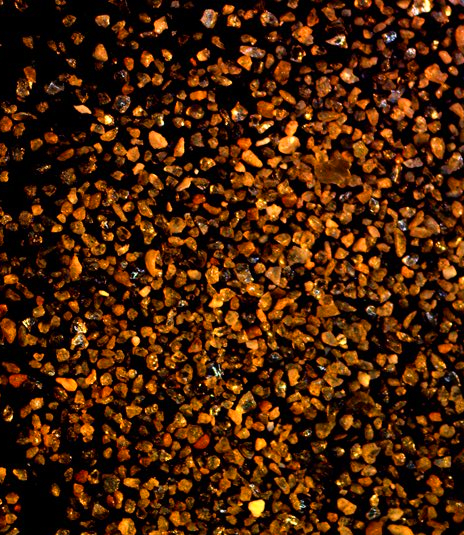
\includegraphics[height=\paperheight]{front.jpg}}; % Background image
\draw[anchor=north] (midpoint) node [fill=ocre!30!white,fill opacity=0.6,text opacity=1,inner sep=1cm]{\Huge\centering\bfseries\sffamily\parbox[c][][t]{\paperwidth}{\centering Vision Soil Analyzer\\[15pt] % Book title
{\Large Product design of a vision based soil analyzer}\\[20pt] % Subtitle
{\huge Jelle Spijker}}}; % Author name
\end{tikzpicture}};
\end{tikzpicture}
\vfill
\endgroup
\newpage
~\vfill
\thispagestyle{empty}

\noindent Copyright \copyright\ 2015 Jelle Spijker\\ % Copyright notice
\noindent \textsc{Published by Royal IHC}\\
\\ % Publisher
\noindent \textsc{www.ihcmerwede.com}\\
\noindent \textsc{www.mtiholland.com}\\
\noindent \textsc{www.han.nl}\\

\noindent This document remains the property of “IHC Holland B.V.” All rights reserved. This document or any part thereof may not be made public or disclosed, copied or otherwise reproduced or used in any form or by any means, without prior permission in writing from “IHC Holland B.V.” \\ % License information

\noindent \textit{First printing, September 2015} % Printing/edition date

\chapterimage{sand_1_banner.jpg} % Table of contents heading image

\pagestyle{empty} % No headers

\tableofcontents % Print the table of contents itself

\cleardoublepage % Forces the first chapter to start on an odd page so it's on the right

\pagestyle{fancy} % Print headers again

\chapter{Introduction}
This project finds its roots in the minor Embedded Vision Design @ HAN, hereafter named EVD. During this minor an embedded device was developed which analyses soil samples using a microscope. This Vision Soil Analyzer hereafter refereed to as VSA, analyzes samples using the optical properties. It gives an user information on color, texture and structure.

This is developed in collaboration with Royal IHC and MTI Holland. Royal IHC is one of Holland major shipyard companies and specializes in dredging and offshore. MTI Holland BV is royal IHC dredging knowledge center. They're worldwide leading centre of expertise in the area of translating knowledge of dredging, mining and deep-sea mining processes into the specification, design and application of equipment.

Both companies have an interests in knowing the properties of soil, be it to advise their customers or to further facilitate their own research and services. Current methods, like the Particle Size Analysis using a sieve and hydrometer are time consuming and non portable. To facilitate quick, accurate and on location soil research an embedded device has been developed. This VSA analyzes soil samples using a microscope and gives the user acceptable and quick results on the soil visual properties.

Quick and reliable results are a welcome addition into any laboratory, this combined with a device that is light and portable gives it's users an added benefit of shortened logistical operations for their soil samples. This results in some serious time benefits.

During the first period of the minor a basic prototype has been developed. This prototype ran in Matlab on a X64 desktop computer and was a first test case for the algorithms and idea's. In the second period this prototype is developed on an ARMv7 embedded Linux device and is compiled in C++. The goal of the software is to analyze soil samples and presenting the user with information regarding it's color, texture and structure.

Information regarding the color of a sample is presented to the user in the CIE Lab and Redness Index color-models. These color models show correlation between different soil properties, such as iron content and fertility. Conversion between different color-models are CPU intensive, because each pixel will be transformed using multiple algorithms. It's therefore paramount that calculations are done with an minimum of machine instructions and with acceptable errors.

Texture information is presented to a user via a Particle Size Distribution, hereafter named PSD. This is a cumulative function representing the ratio of different particle sizes in the soil sample. Due to the nature of a two dimensional digital image numerous problems arise. These are overlap of smaller particles by bigger particles, this gives a distortion in the PSD results, because the smaller particle is registered as part of the bigger particle. And another problem is the fact that soil particles are three dimensional. but the image is two dimensional.

Information about the structure of the soil is extrapolated from the individual particles shapes. These shapes are describes in the frequency domain, using a Fast Fourier Transform and fed into a Neural Network which classifies these shapes into standard soil categories. These are time consuming operations and therefore should be done with a minimum of machine instructions and efficient programming.

This wiki / product documentation gives the developer(s) and customers, namely MTI and IHC a tool to further the development of the VSA in to a full fledge market ready product. The development environment and the used protocols are described in order to guard the quality of the work. The product itself is designed by determining a global IPO Input-Process-Output diagram. This leads to the functional specifications. To illustrate the working of the device further the User Interface will be designed which will be supplemented with a short manual. All the above design tools will come together in a detailed IPO. Correct working of the device is guaranteed with various testing protocols. The current working principles follows a set global workflow. The vision related algorithms are describe in order to determine the most efficient working order. This results in the complete image processing steps

The following project setup is proposed for the release candidate. Future release will follow the roadmap

\newpage
\part{Design}

\chapterimage{sand_2_banner.jpg} % Chapter heading image
\chapter{Functional Design}

\section{Global Input-Proces-Output}\index{Global Input-Proces-Output}
\paragraph{Global workflow}
The soil sample is dried and the user makes sure the particle don’t bond together. A small portion of the sample is placed on a sample plate. Taking care to separate the individual particles as much as possible. The cover is closed and a microscopic camera is positions, in an environment where the light conditions are controlled.

The embedded Linux device takes a snapshot which is analyzed using the following computer algorithms: First the individual soil particles are identified in the image, using various algorithms, such as adaptive contrast stretch, Gaussian blurring, OTSU – optimal thresholds separation. The color information is determined with various matrix calculations, translating the RGB pixel value tot CIE Lab and Redness Index.

The texture information is determined by counting the number of discrete pixels for each individual article. From this the volume is determined. If the scale of each pixel is known, the volume can be given in SI units.

The structure of an individual particle is determined by getting the edge of the pixels. This is done by creating a mask with a morphological erosion algorithm this mask is subtracted of the original image. The contour is translated to a function using the Dijkstra shortest path algorithm. Where each pixel is described as an imaginary complex number representing the radius towards the center of the particle. The vector holding these values are transformed to the frequency space using the Fast Fourier Transformation. The describing complex numbers gained during this transformation are fed into a feedforward Neural Network, which is optimized using Genetic Algorithms and a previously determined learning data set. The output is presented as probability that a certain particle belongs to a predefined category.

The results are presented to the user via a graphical user interface which are show when the device is hooked to a monitor carrying a HDMI input. It’s also possible to present a report in pdf or a native format which can downloaded from the device using a LAN network device or optional Wi-Fi or Bluetooth. Basic human interaction can be performed via an on-board encoder, or optional USB keyboard and/or mouse.
\paragraph{Technical system}
\begin{sBox}
	Prototype of an intelligent soil microscope
\end{sBox}

\paragraph{Main function}
\begin{sBox}
	To analyses a dried soil sample, consisting of particle in the range of $ 0.02 [mm] leq P leq 2.0 [mm] $ and present a user with information regarding color, texture and structure.
\end{sBox}
\section{Specifications}\index{Citation}


\subsection{Functional requirements}
\begin{description}
	\item[Name] Description
	\item[Word] Definition
	\item[Comment] Elaboration
\end{description}
\subsection{Technical requirements}
\begin{description}
\item[Name] Description
\item[Word] Definition
\item[Comment] Elaboration
\end{description}

\chapter{User Interface}

\section{Graphical User Interface}

\begin{figure}[h]
	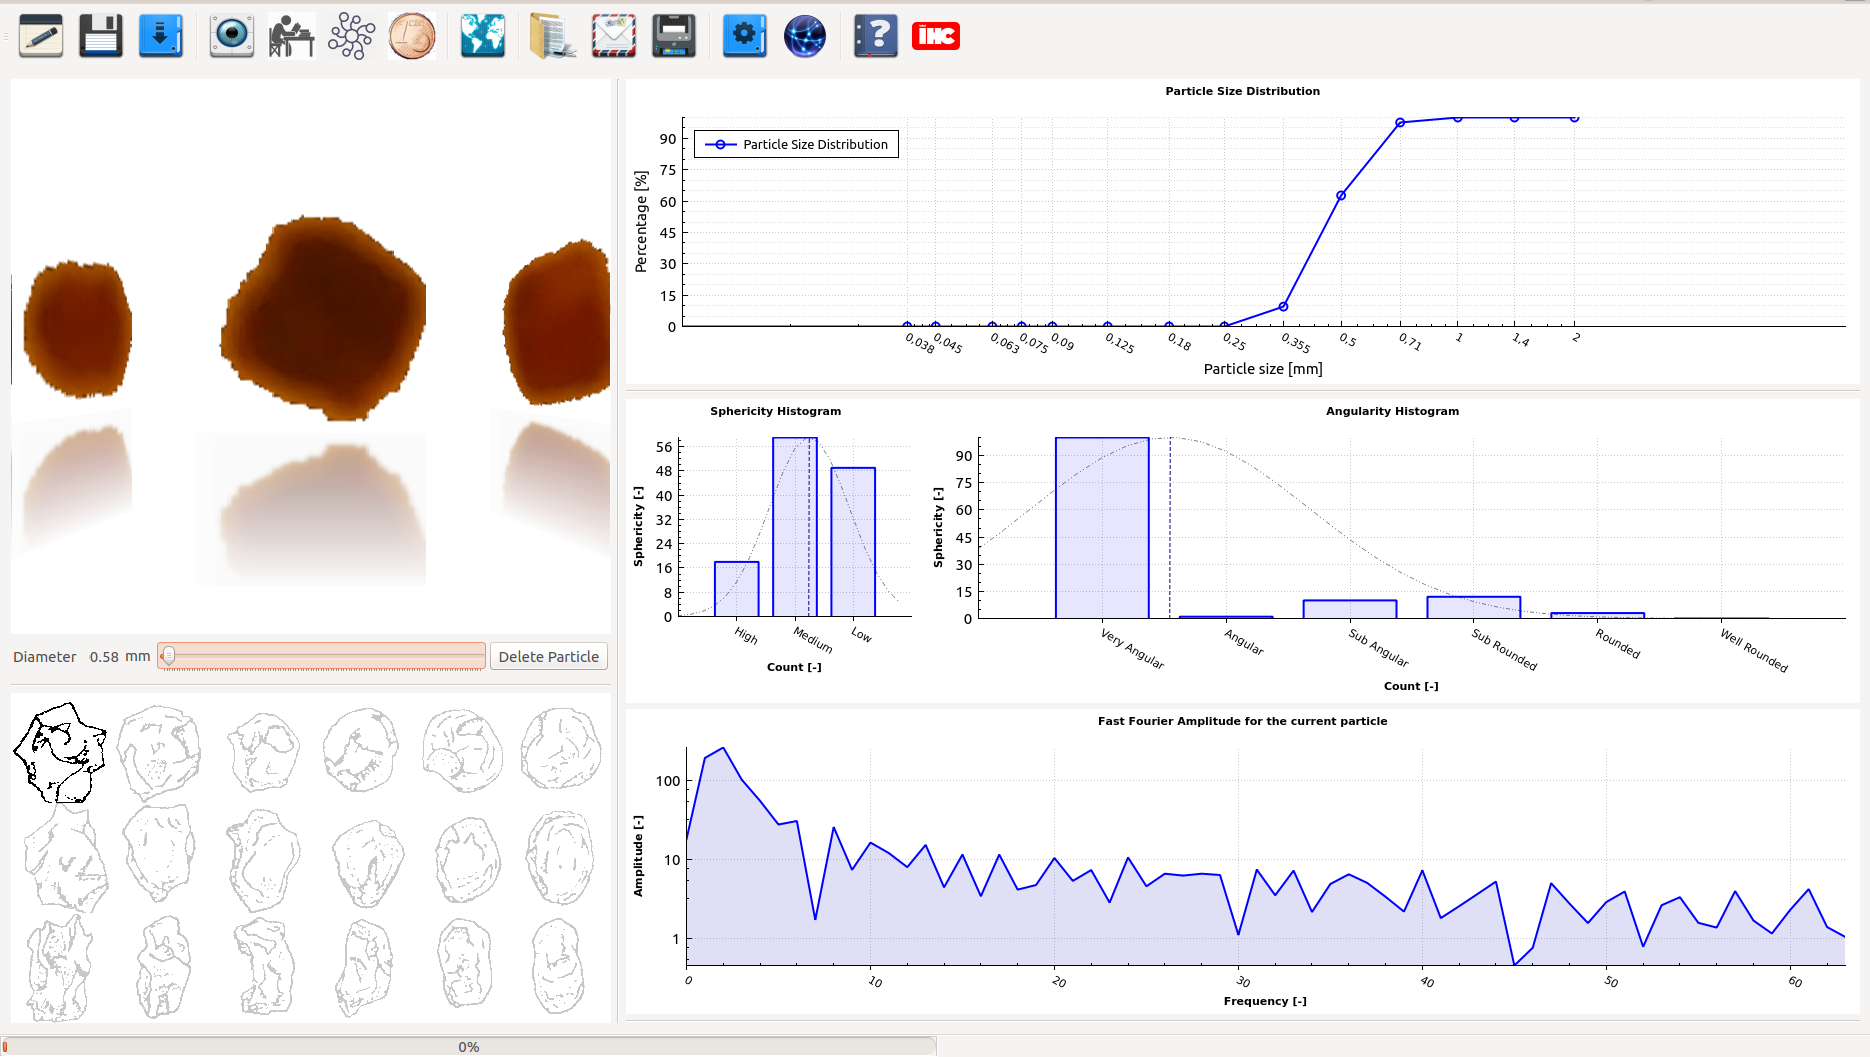
\includegraphics[width=\textwidth]{maingui.png}
	\caption{Main Graphical User Interface}
\end{figure}


\section{Hardware User Interface}

\chapter{Manuals}

\section{User manual}

\section{Administrator manual}

\chapter{Technical Design}

\section{Hierarchical structure} \index{Hierachical structure}

This is an example of theorems.

\section{Architecture} \index{Architecture}
This is a theorem consisting of several equations.

\section{Detailed Input-Process-Output schematics} \index{IPO}
This is a theorem consisting of just one line.

\subsection{Led driver}

\subsection{Global position unit}

\subsection{Controller}

\chapter{Vision design}

\part{Realization}

\chapterimage{sand_3_banner.jpg} % Chapter heading image
\chapter{Technical Realization}

\subsection{Electrical design}

\subsection{Design}

\chapter{Vision realization}
This chapter describes the used vision processing techniques. The current prototype and work flow is developed to allow for different routines. The user has multiple options and strategies available to achieve optimum results. Each of these are explained in the sequential subsection below. It begins with the acquisition of image(s), which are then enhanced to allow for optimal segmentation of pixels related to sand particles. These pixels are used to determine the features of each particle, which serve as input for the classification algorithms.

\section{Image acquisition}\index{Acquisition}
A thorough review of the current literature \cite{Spijker14a} identified three properties that can be used in vision based analyzing. These properties are structure \index{structure} (shape), color and texture \index{Texture} (size). When looking closely at sand sample, you notice a multitude of shapes, colors and sizes, each particle is unique and differs from its neighbor. This diversity brings it own challenges. The shape of a particle determines how it will rest on the sample plate. The color and the translucency of the particle, determines how easily it can be segmented or identified from the background. Whilst the size determines the needed focus depth of the microscope. 
\begin{remark}
	In samples, where the particles show a huge spread in size, compared to the mean size, there will be a noticeable difference in focus, between big and small particles. 
\end{remark}

\paragraph{Acquisition strategies}The first prototype is developed in such a way that multiple acquisition strategies\index{acquisition strategies} can be implemented. Each of these tackle different challenges. The quality of the acquired image is the biggest factor in the successful extraction of a particle, but in order to make any valid claim about the sample, a certain amount of particles have to examined. To determine the minimum sample size \index{Minimum sample size}, the following equation can be derived:
\begin{sBox}
	Let the reliability be $95\% \therefore z=1.96$, the probability be $P=50\%$ and the accuracy be $\alpha=5\%$; consider the function:
	\begin{equation}
		z\sqrt{\frac{p\times(1-P)}{n}}\leq\alpha \rightarrow n\geq\frac{-p\times(P-1)\times z^2}{\alpha^2}
	\end{equation}
\end{sBox}
This brings the minimum amount of particles to $384$. With the predefined range of particle sizes ($0.2[mm]\leq P_size \leq 2[mm]$ where $P$ defines a particle) and the limited work area under the microscope, multiple shots have to be taken. Where the sample is rearranged. Between fifteen and twenty shots are usually enough.
\begin{remark}
	The process of rearranging the particles, will be automated in the future. Student of the minor Offshore \& Construction taught at the University of Applied Sciences Rotterdam will work on this challenge. This is done on the RDM Campus. This minor starts in September 2015. Their product will serve as input for the second prototype. Their assignment is described in appendix \ref{RDM_Campus} and will be executed under the auspice of MTI Holland and the author.
\end{remark}

\paragraph{Acquisition} \index{Acquisition} Each sample is placed in a light condition room, and laid out on a semitransparent white acrylate plate. The sample can be illuminated with a bright field light source, where the light is aimed directly at an object or the particle can be lit with back lighting. See the course notes \cite{ypma_course_2014} for a more in-depth description. The choice for back lighting can be made because translucent particle are harder to segment in a bright field light. The trade off is extra processing time.

After the sample is placed in the light condition room, the microscope takes a image with bright field illumination \index{Bright field illumination} and, if the option is selected, another one with back lighting. \index{Back lighting} Hereafter the sample is rearranged, this is a manual procedure. Once the sample is rearranged a new set of shots is taken. Each image that is acquired from the microscope is defined by a matrix were the values are triples for the RGB \index{RGB} (red, green and blue) values and these are defined by an unsigned byte. 

Each image is stored in a vector using a custom container. This container consists of a bright field image, back light image and a SI-conversion factor \index{SI-conversion factor}. Each time the height is changed, the microscope has to be calibrated so that the relation between pixel and [mm] can be determined. This is done by taking a shot of a disc with known dimensions. A single euro cent can serve for this purpose.

\begin{remark}
	The image is stored in the OpenCV matrix (cv::Mat) container. This container is  designed to handle image processing data and routines. It makes use of memory management and smart pointers to handle the data effectively. 
\end{remark}

\section{Image enhancement}\index{Enhancement}
Image enhancement prepares the RGB image for conversion to a binary image. It eliminates noise and brings out wanted features, by using filters.
\paragraph{Intensity image}\index{Intensity image}\label{IntensityImg} The first step in this process step is the conversion from the RGB color space to an scalar valued image which represent the luminosity, also known as a intensity image. This luminosity is calculated using a weighted average and is done for bright field and back lit images.
\begin{sBox}
	Let $\mat{I}$ and $\mat{R}, \mat{G}, \mat{B}$  be a matrices with dimensions $n \times m$ derived from the color matrix $\mat{RGB}$ with dimensions $n \times m \times 3$; The weighted average can be calculated with the following equation:
	\begin{equation}
		\mat{I} =0.2126\times \mat{R} + 0.7152\times \mat{G} + 0.0722\times \mat{B}
	\end{equation}
\end{sBox}

\paragraph{Adaptive contrast stretch}\index{Adaptive contrast stretch}\label{Adaptive contrast stretch} After the conversion from RGB to an intensity image, the user has the choice to apply an adaptive contrast stretch to the bright field images. This process is used to enhance the contrast of the intensity image. For every pixel and its surrounding area the mean and standard deviation are calculated. If the value of the pixel is above or below the mean than the following rule is used to determine the new value: $\mat{I}_{n,m}=\mat{I}_{n,m} \times \alpha \pm \sigma$, where $\alpha$ is a scaling factor and $\sigma$ is the standard deviation of the old pixel value with it's neighboring kernel pixels.

\paragraph{Blur}\index{Blur}\label{Blur} As a second enhancement the user can apply a blurring operation to the bright field images, in essence the opposite of the contrast stretch. The blur operation also determines the mean for every pixels within a given area: the kernel. The mean value of the kernel is assigned to the pixel.

\paragraph{Cropping}
The above operations described in the paragraph \ref{Blur} and \ref{Adaptive contrast stretch}, leave the border pixels unaffected in their calculations. This offset is determined by half of the biggest kernel size. These pixels are discarded for the next step. The enhanced intensity matrix is used for particle segmentation, see section \ref{Segmentation}. Whilst the intensity matrix of the bright field image is used for the conversion to the CIE La*b* colorspace, as explained in section \ref{CIELab}.

\section{Feature extraction}\index{Feature extraction}\label{Segmentation}
In order to tell something about the individual particles, they first have to be identified and separated from the background. This is done with the enhanced intensity matrix. Which is taken from the bright field matrix or if available the back lit intensity matrix.

\paragraph{Segmentation}\index{Segmentation}
The images are segmented by calculating a threshold value\index{Threshold}. This value is determined by using the Otsu\index{Otsu's method} threshold. \citeauthor{Xu2011956} \cite{Xu2011956} describe that the Otsu threshold is equal to the average of the mean levels of two classes partitioned by this threshold. This threshold can be iteratively determined.

\begin{sBox}
	Let $\vec{h}$ be a vector of dimension $256$ which represent a count of values in the enhanced intensity matrix $\mat{I}$ with dimensions $m \times n$
	\begin{equation}
		\frac{1}{t}\sum\limits_{i=1}^t \vec{h}_i = t - \frac{1}{256-t}\sum\limits_{i=t}^{256} \vec{h}_i
	\end{equation}
\end{sBox}

\subsection{CIE La*b* extraction}\index{CIE La*b*}\label{CIELab}

\subsection{Fast Fourier Descriptors}\index{Fast Fourier Descriptors}\index{FFT}\label{FFT}

\subsection{Particle Size Distribution}

The normal procedure for creating a Particle Size Distribution uses sieves and weights, to determine the volume of the the particle.

The Sieve mesh size can be perceived as a cross section of a particle, since the particle is only retained in a sieve when it passes through the top sieve but can't pass through the sieve below. The cross section of the particle is at minimum the sieve mesh size of the top sieve, but other dimensions of the particle can exceed the sieve mesh size at which it last passes.

[Work this argument to explain why it's oke to use a 2 dimensional representation of a 3 dimensional particle]

\section{Classification}\index{Classification}

\subsection{Roundness using Hu-moments}\index{Roundness} \index{Hu-moments}\label{HuMoments}

\subsection{Angularity using a Neural Network}\index{Angularity} \index{Neural Network}\label{NeuralNet}
Angularity of particle can be described as 


\begin{figure}[h, center]
	\begin{center}
		\begin{neuralnetwork}[height=4, nodespacing=40]
				\newcommand{\nodetextclear}[2]{}
				\newcommand{\nodetextx}[2]{$FFT_#2$}
				\newcommand{\nodetexty}[2]{$Class_#2$}
				\inputlayer[count=4, bias=false, title=Input layer, text=\nodetextx]
				\hiddenlayer[count=5, bias=false, title=Hidden layer, text=\nodetextclear] \linklayers
				\outputlayer[count=3, title=Output layer, text=\nodetexty] \linklayers
		\end{neuralnetwork}
	\end{center}
	\caption{Neural Network}
\end{figure}


\subsection{Genetic Algorithm}

\paragraph{Viva la revolution!}

This is an example of examples.

\part{Verification}

\chapterimage{sand_4_banner.jpg} % Chapter heading image

\chapter{Presenting Information}

\section{Table}\index{Table}

\begin{table}[h]
\centering
\begin{tabular}{l l l}
\toprule
\textbf{Treatments} & \textbf{Response 1} & \textbf{Response 2}\\
\midrule
Treatment 1 & 0.0003262 & 0.562 \\
Treatment 2 & 0.0015681 & 0.910 \\
Treatment 3 & 0.0009271 & 0.296 \\
\bottomrule
\end{tabular}
\caption{Table caption}
\end{table}

\section{Figure}\index{Figure}

\begin{figure}[h]
\centering
\includegraphics[scale=0.5]{placeholder}
\caption{Figure caption}
\end{figure}

\part{Addenda}

\chapterimage{books_banner.jpg}
\chapter*{Bibliography}
\addcontentsline{toc}{chapter}{\textcolor{ocre}{Bibliography}}
\section*{Books}
\addcontentsline{toc}{section}{Books}
\printbibliography[heading=bibempty,type=book]
\section*{Reports}
\addcontentsline{toc}{section}{Reports}
\printbibliography[heading=bibempty,type=report]
\section*{Articles}
\addcontentsline{toc}{section}{Articles}
\printbibliography[heading=bibempty,type=article]

\chapterimage{Index_banner.jpg}
\cleardoublepage
\phantomsection
\setlength{\columnsep}{0.75cm}
\addcontentsline{toc}{chapter}{\textcolor{ocre}{Index}}
\printindex

\appendix
\chapterimage{books_banner.jpg}
\chapter{Graphical User Interface}
\begin{figure}[h]
	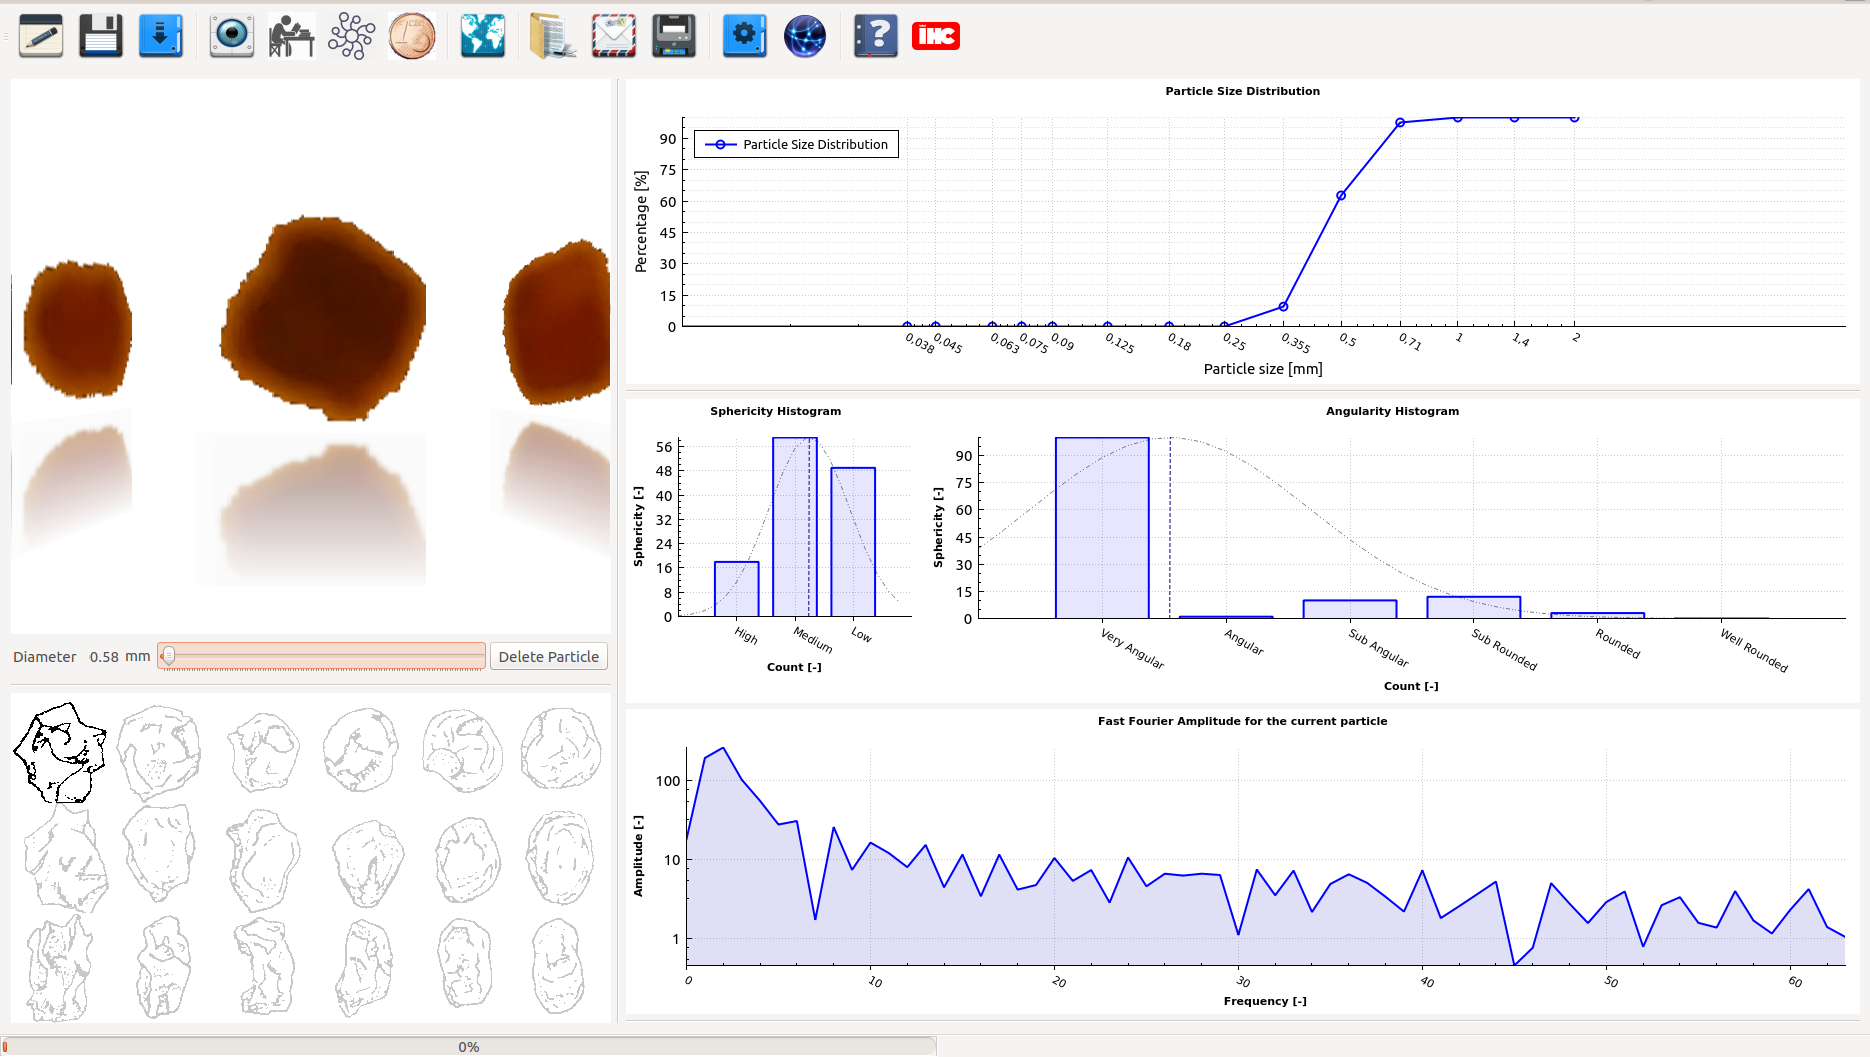
\includegraphics[width=\textwidth]{maingui.png}
	\caption{Main Graphical User Interface}
\end{figure}
\begin{figure}[h]
	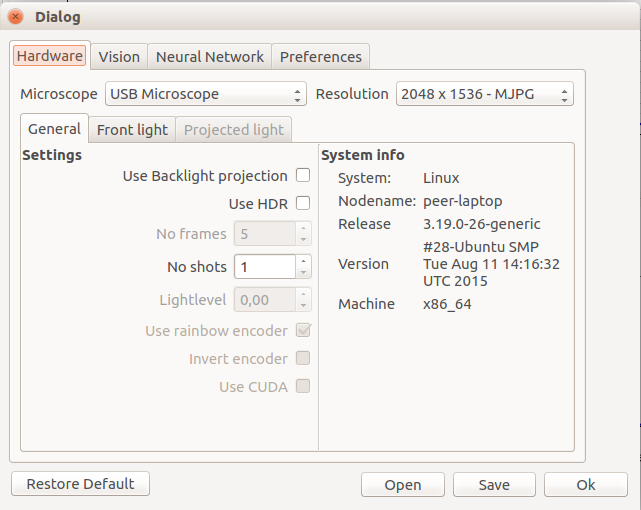
\includegraphics[width=\textwidth]{settingHardware.png}
	\caption{Settings Hardware Interface}
\end{figure}
\begin{figure}[h]
	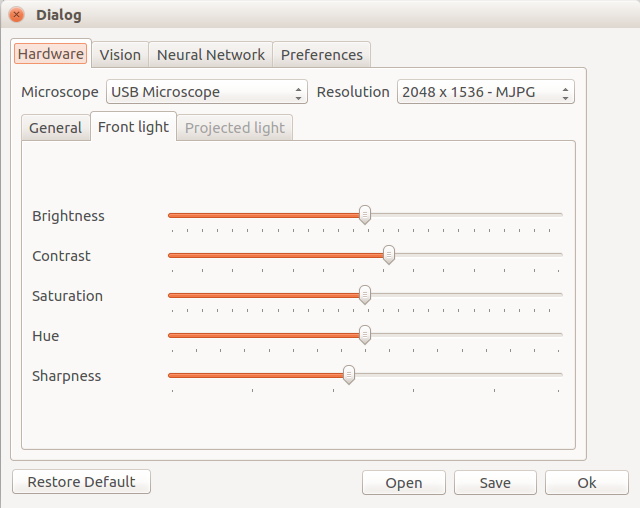
\includegraphics[width=\textwidth]{settingsHardwareCam.png}
	\caption{Settings Hardware Cam Interface}
\end{figure}
\begin{figure}[h]
	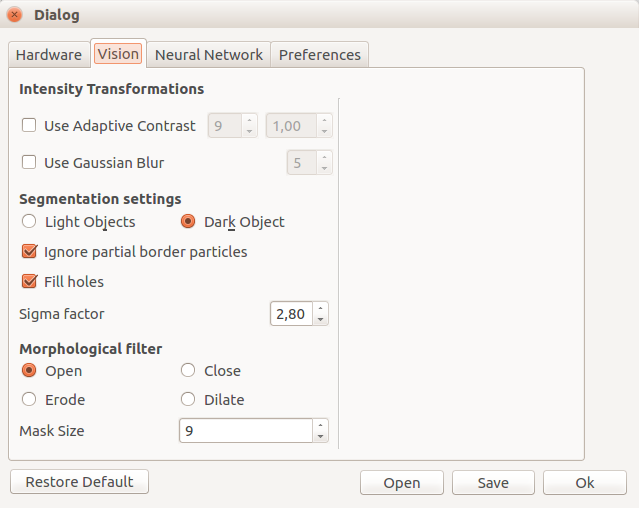
\includegraphics[width=\textwidth]{settingsVision.png}
	\caption{Settings Vision Interface}
\end{figure}
\begin{figure}[h]
	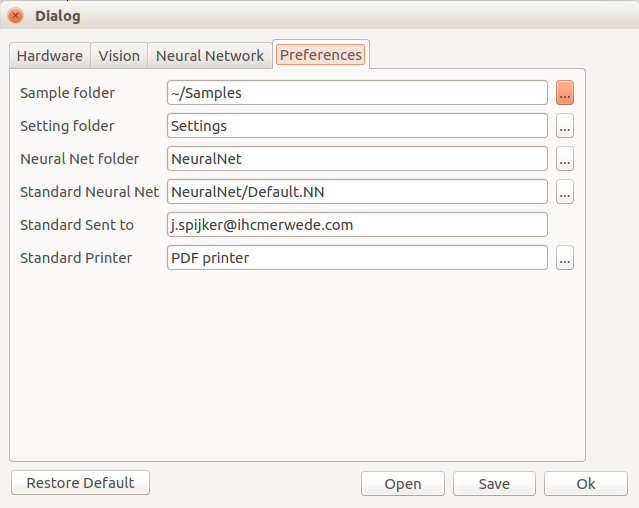
\includegraphics[width=\textwidth]{settingsPref.png}
	\caption{Settings Preference Interface}
\end{figure}
\begin{figure}[h]
	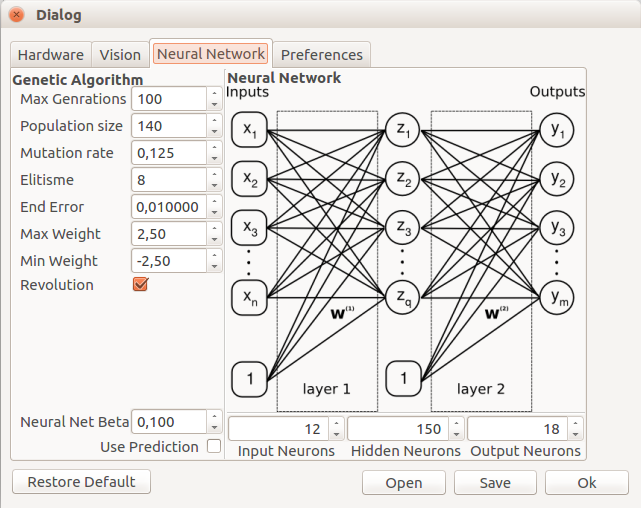
\includegraphics[width=\textwidth]{settingsNN.png}
	\caption{Settings Neural Network Interface}
\end{figure}
\begin{figure}[h]
	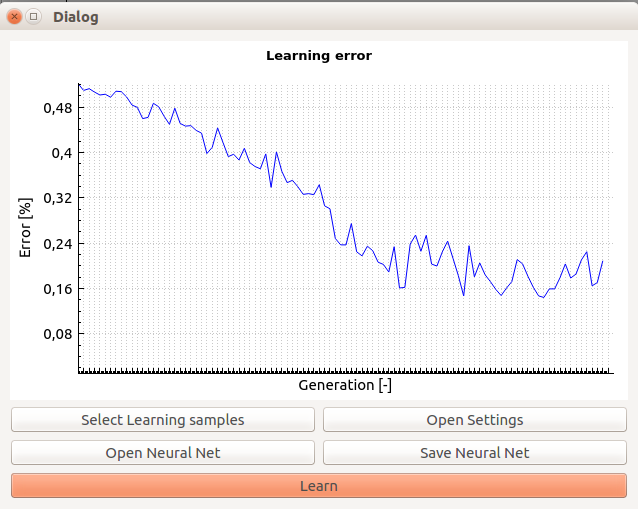
\includegraphics[width=\textwidth]{NNLearn.png}
	\caption{Neural Network Learning Interface}
\end{figure}

\chapter{Example Soil Report}
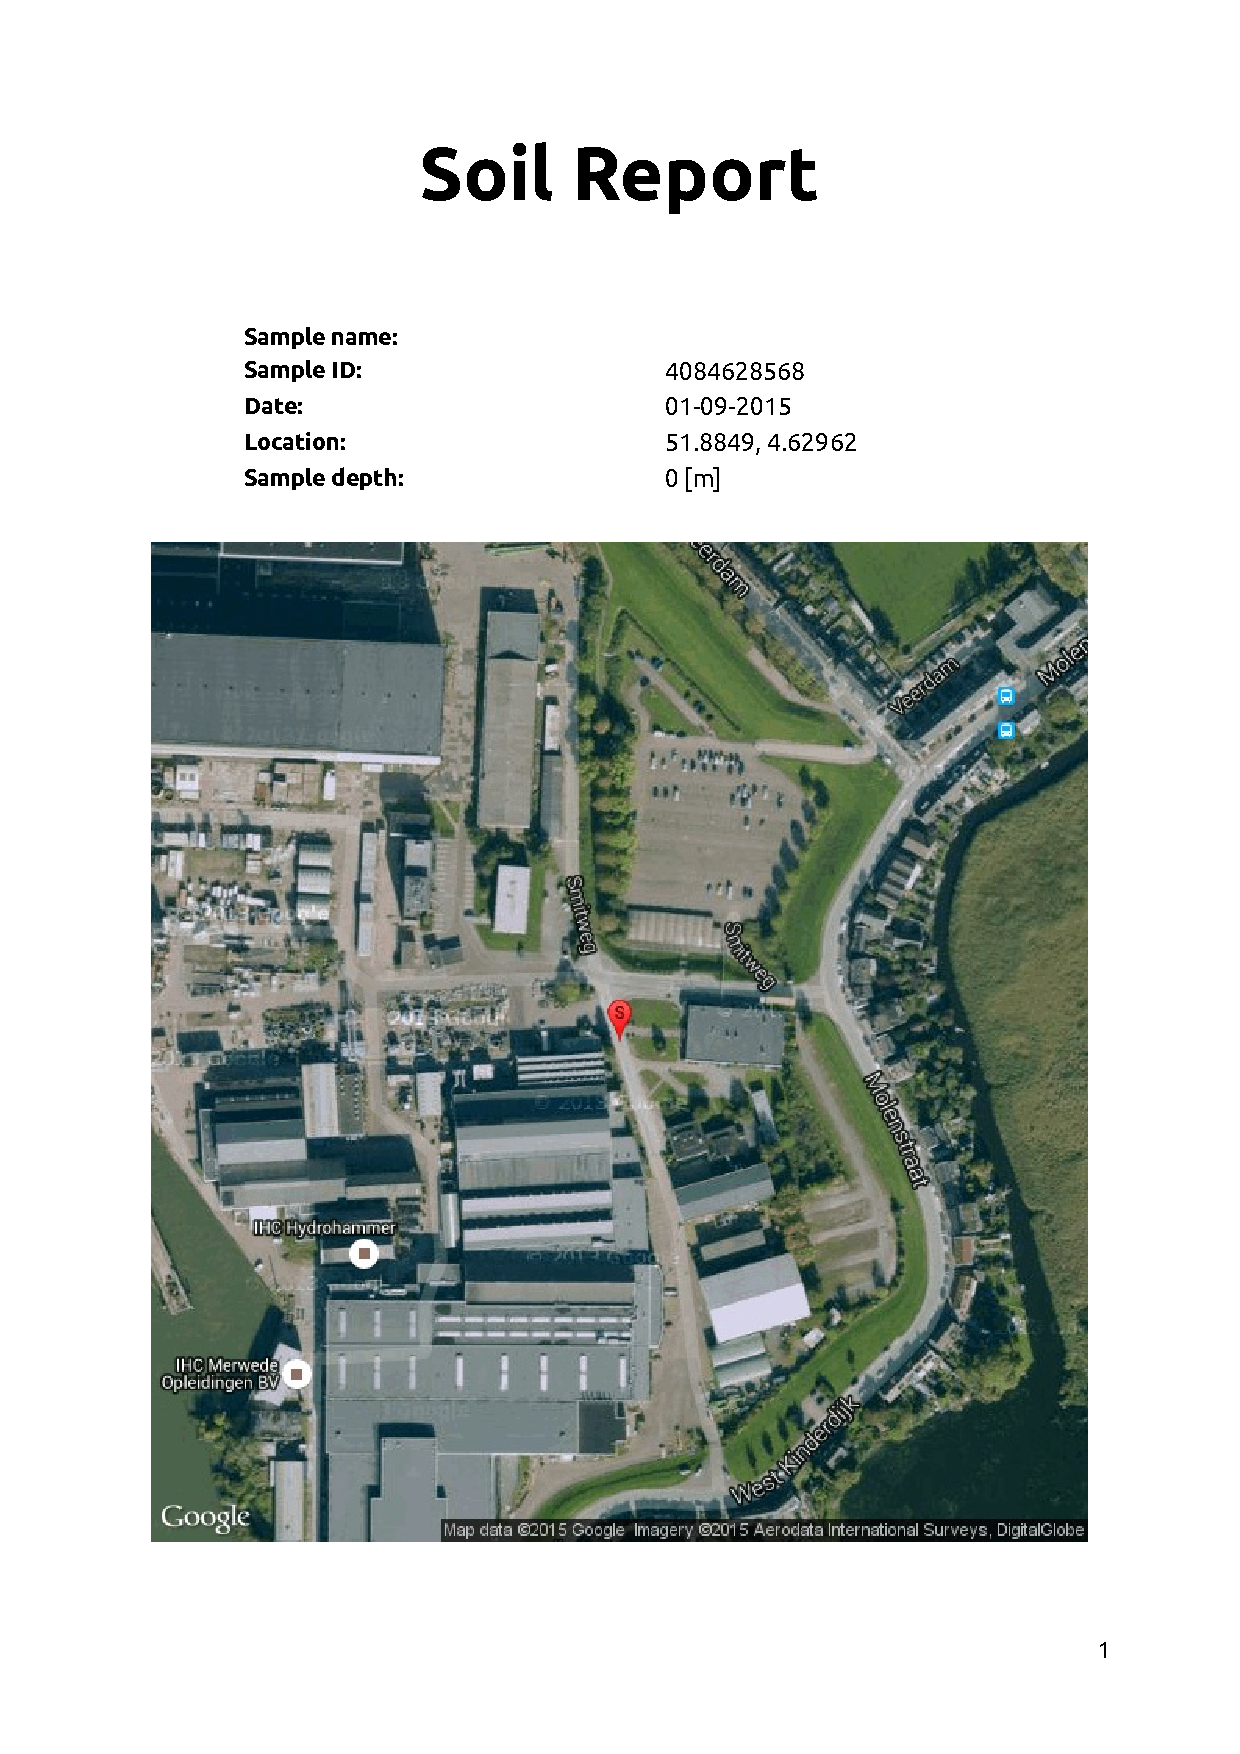
\includepdf[pages={1-5}, height=\textheight ,pagecommand=\paragraph{}]{SampleReport.pdf}

\chapter{RDM campus: Student project}\label{RDM_Campus}
Subject: RDM Student project\\
Author: Jelle Spijker\\

\paragraph{Introduction}
This project finds its roots in the minor Embedded Vision Design (EVD) taught at the university of applied sciences HAN. During this minor a portable embedded device was developed which analyses soil samples using a microscope. This Vision Soil Analyser hereafter referred to as VSA, analyses soil samples using the optical properties. It’s main function is: Presenting quantifiable information to a user on the properties of soil: such as colour, texture and structure.

The VSA takes a snapshot from a soil sample, which is placed under a microscope in an closed environment. This digital image is analysed using a multitude of computer vision algorithms. Statistical data is presented to the user in the form a Particle Size Distribution (PSD) and a histogram of the shape classification. The PSD is obtained by calculating the number of pixels for each individual particle, whilst shape classification is determined by describing the contour of each individual particle as mathematical function which undergoes a transformation to the frequency domain. This complex vector then serves as input for an Artificial Neural Network (ANN) where the output classifies each particle in a certain category.

The prototype developed during the minor EVD will serve as a basis for a graduation project of that same student, which initialized the project. This is done for his main course mechanical engineering at the HAN. This graduation project is done under the auspices of MTI Holland. The goal during this second stage is to develop a field ready prototype. In conjunction with the necessary documentation (Technical Dossier). 
Due to the scale of the project, several key problems are identified and separated from the main project. These problems can be tackled by separated student groups.

\paragraph{Problem description}
Due to the transformation from 3D particles to a discrete 2D image certain data is lost. This degradation of data introduces errors in the statistical data. One of the forms of degradations is the overlap of bigger particle onto smaller particles. These particles are identified as an particle with at least the size and the contour of the biggest particles. Thus giving false negatives for the smaller particles and often false positives for the bigger particle.

A solution that will be explored during this stage is the execution of multiple analysis of the same discrete particle population. This will result in an accurate statistical representation of the soil sample placed under the microscope.

The project that the RDM students can tackle can be described as follow:
\begin{sBox}
	Design and build a prototype with which the placement of particles, relative to each other and ranging in sizes from 0.02 - 2 [mm] are randomly changed in a time span of 1 [sec], which is tightly integrated with the main prototype. 
\end{sBox}

The prototype is to be CE compliant and should be build according to technical specifications. It should be described in a Technical Dossier, containing all necessary documents such as: technical drawings (according to mono system), bill of materials, calculation, analysis and design reports.

\chapter{Current project status}
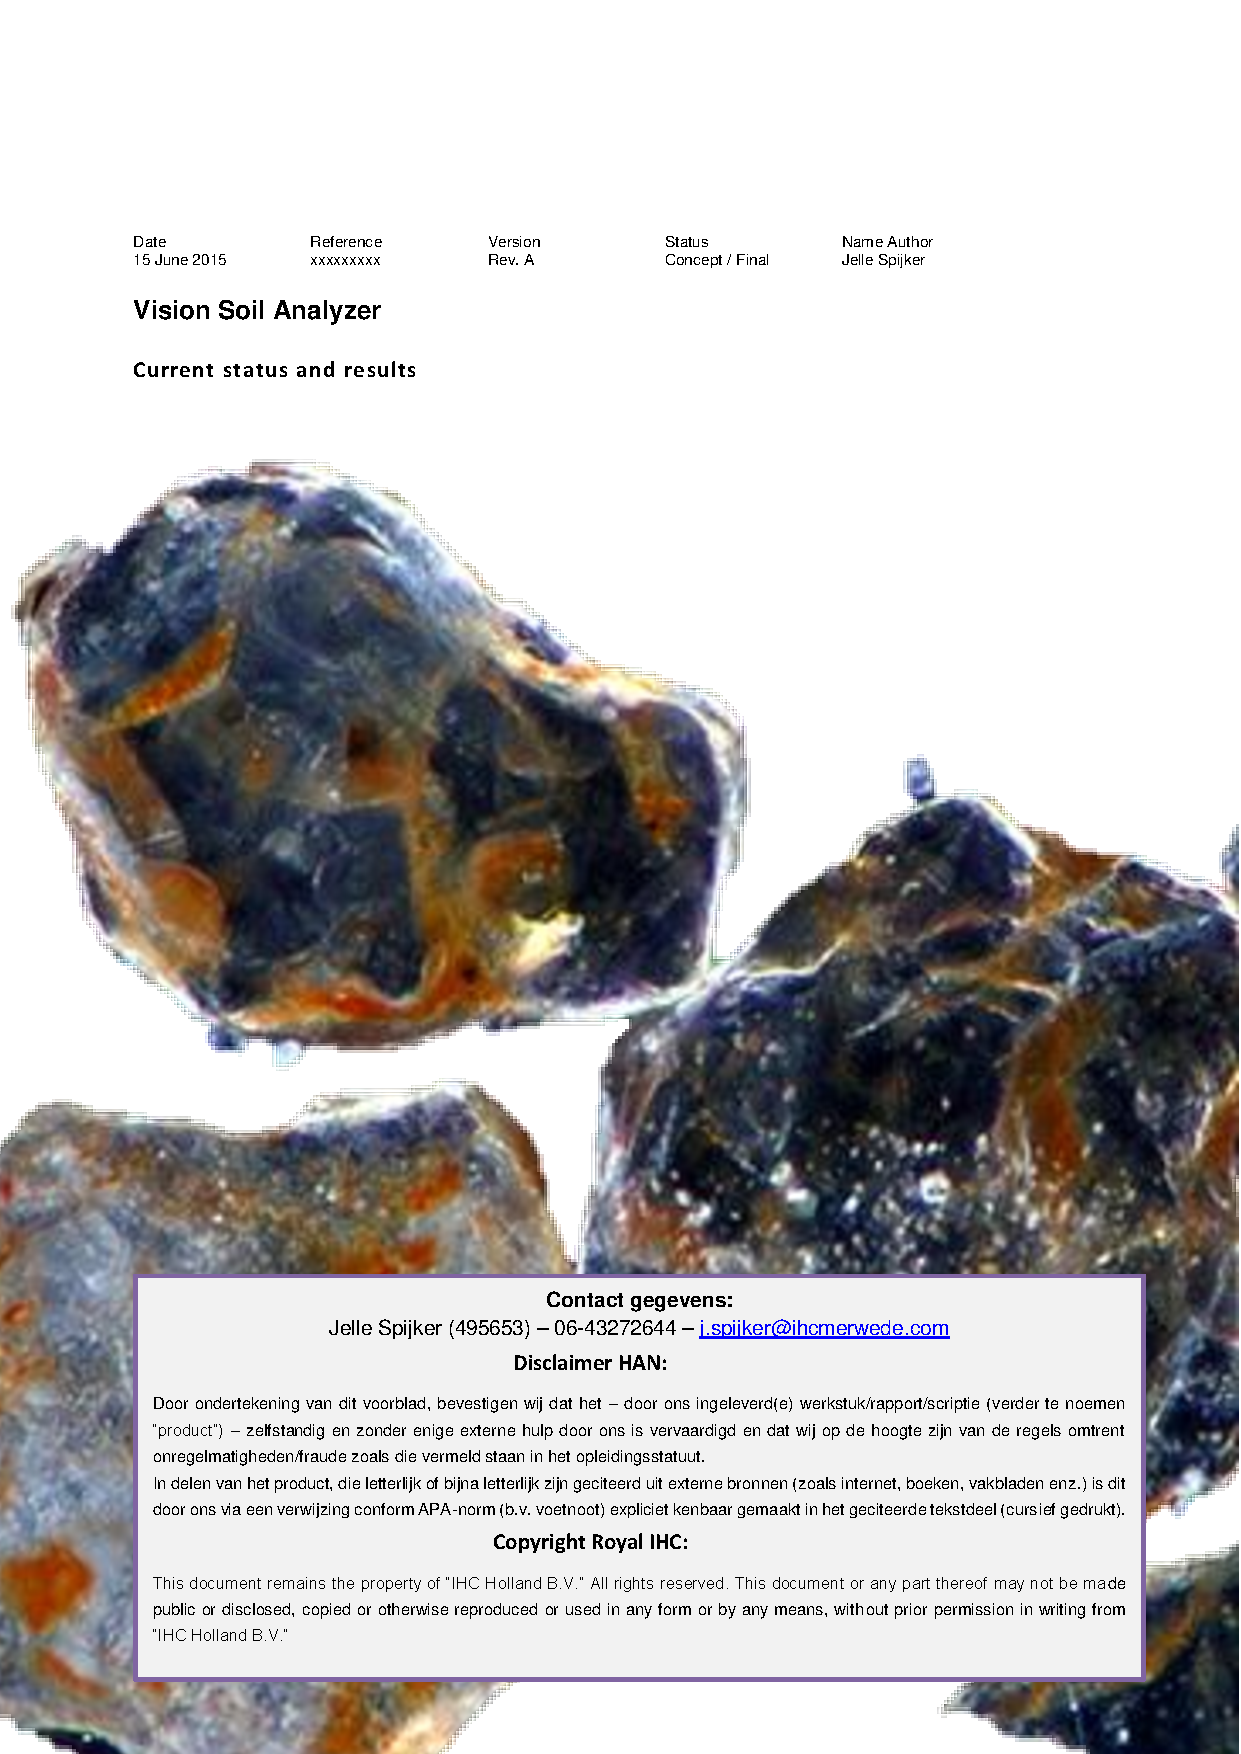
\includepdf[pages={1-7}, height=\textheight ,pagecommand=\paragraph{}]{../IHC/Current Status 150617.pdf}
\chapter{Soil and computer vision flyer}
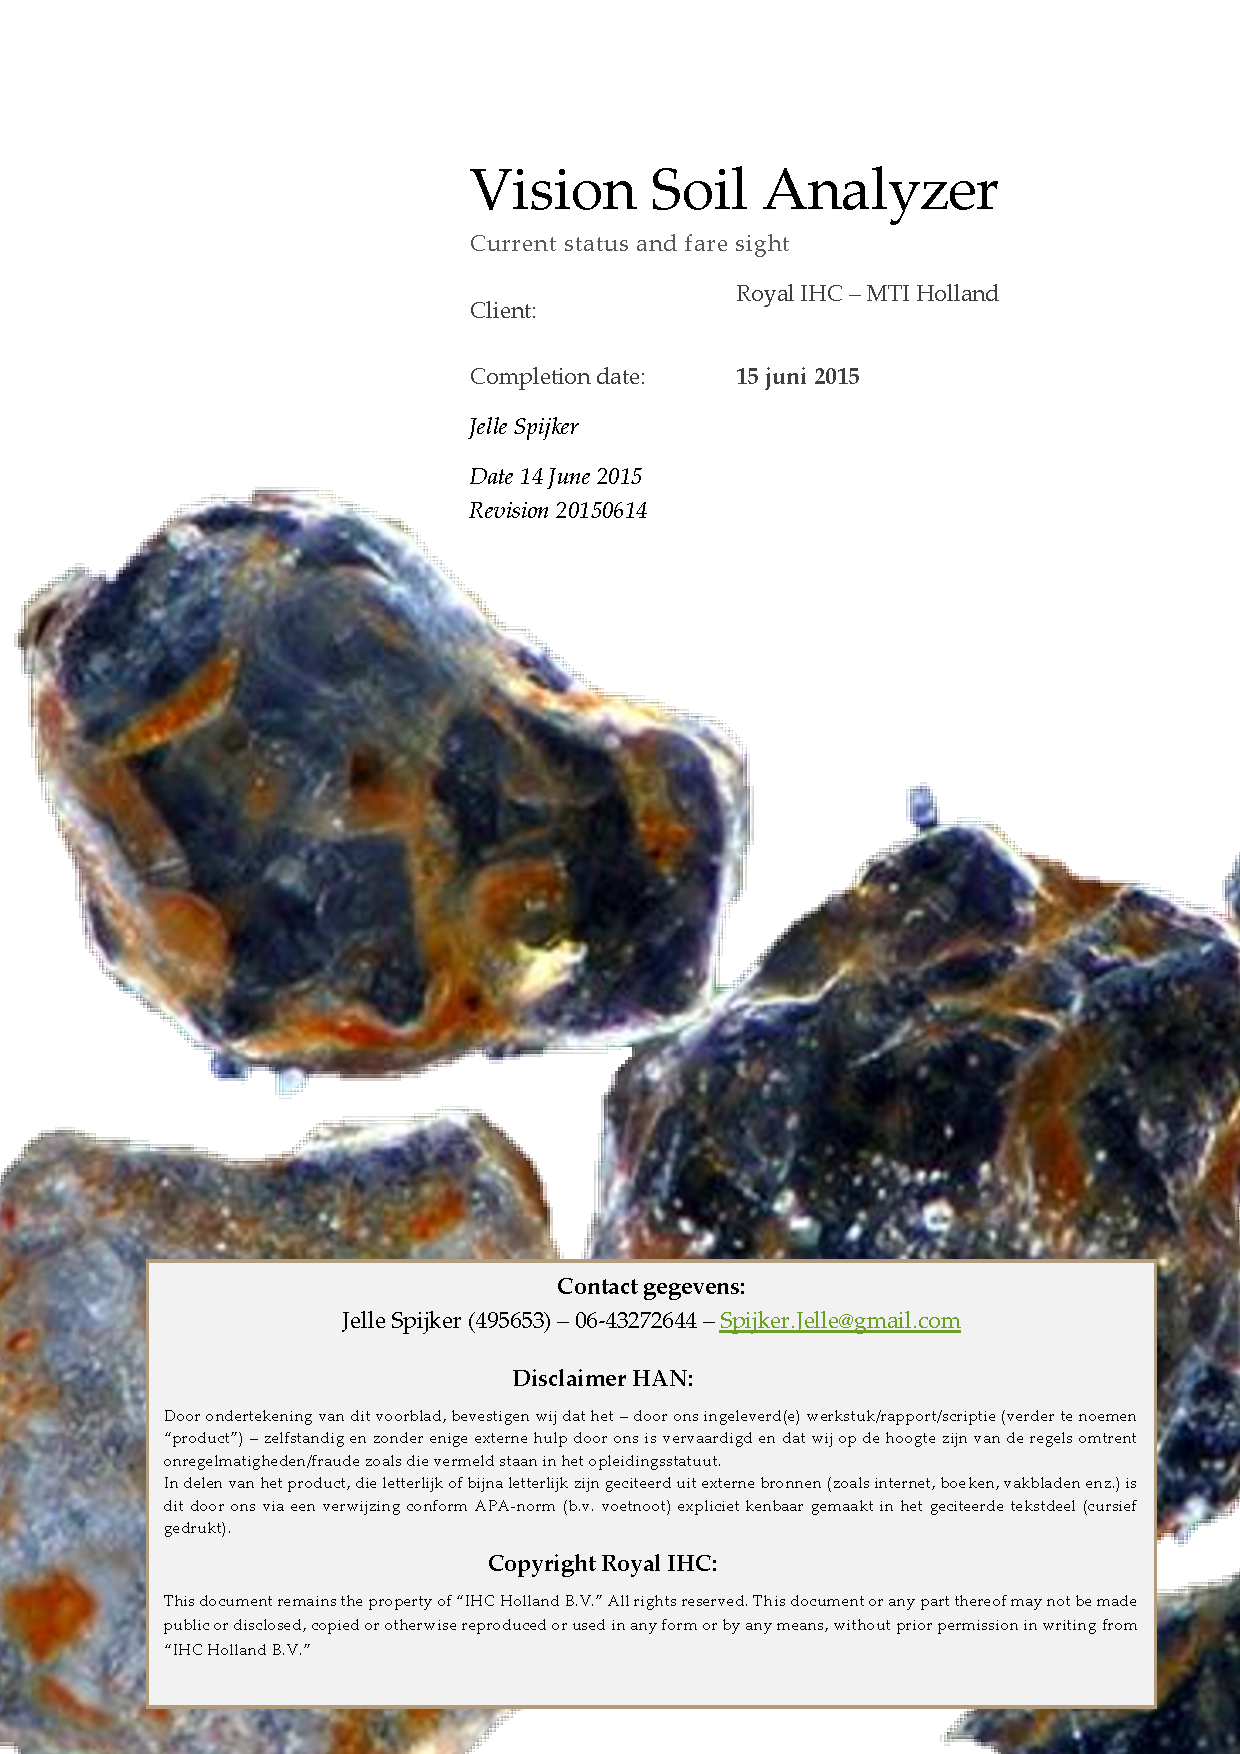
\includepdf[pages={1-15}, height=\textheight ,pagecommand=\paragraph{}]{../IHC/Soil and computer vision.pdf}

\chapterimage{code_banner.jpg}
\chapter{SoilMath Library}
\subsection{Genetic Algorithm Class}
\lstinputlisting[language=C++]{../../src/SoilMath/GA.h}
\lstinputlisting[language=C++]{../../src/SoilMath/GA.cpp}
\newpage
\subsection{Fast Fourier Transform Class}
\lstinputlisting[language=C++]{../../src/SoilMath/FFT.h}
\lstinputlisting[language=C++]{../../src/SoilMath/FFT.cpp}
\newpage
\subsection{Neural Network Class}
\lstinputlisting[language=C++]{../../src/SoilMath/NN.h}
\lstinputlisting[language=C++]{../../src/SoilMath/NN.cpp}
\newpage
\subsection{Statistical Class}
\lstinputlisting[language=C++]{../../src/SoilMath/Stats.h}
\lstinputlisting[language=C++]{../../src/SoilMath/psd.h}
\newpage
\subsection{General project files}
\lstinputlisting[language=C++]{../../src/SoilMath/SoilMath.pro}
\lstinputlisting[language=C++]{../../src/SoilMath/SoilMath.h}
\lstinputlisting[language=C++]{../../src/SoilMath/CommonOperations.h}
\lstinputlisting[language=C++]{../../src/SoilMath/SoilMathTypes.h}
\lstinputlisting[language=C++]{../../src/SoilMath/Mat_archive.h}
\lstinputlisting[language=C++]{../../src/SoilMath/predict_t_archive.h}
\lstinputlisting[language=C++]{../../src/SoilMath/MathException.h}
\lstinputlisting[language=C++]{../../src/SoilMath/Sort.h}

\chapterimage{code_banner.jpg}
\chapter{Hardware Library}
\subsection{Microscope Class}
\lstinputlisting[language=C++]{../../src/SoilHardware/Microscope.h}
\lstinputlisting[language=C++]{../../src/SoilHardware/Microscope.cpp}
\newpage
\subsection{Beaglebone Black Class}
\lstinputlisting[language=C++]{../../src/SoilHardware/BBB.h}
\lstinputlisting[language=C++]{../../src/SoilHardware/BBB.cpp}
\newpage
\subsection{GPIO Class}
\lstinputlisting[language=C++]{../../src/SoilHardware/GPIO.h}
\lstinputlisting[language=C++]{../../src/SoilHardware/GPIO.cpp}
\newpage
\subsection{PWM Class}
\lstinputlisting[language=C++]{../../src/SoilHardware/PWM.h}
\lstinputlisting[language=C++]{../../src/SoilHardware/PWM.cpp}
\newpage
\subsection{ADC Class}
\lstinputlisting[language=C++]{../../src/SoilHardware/ADC.h}
\lstinputlisting[language=C++]{../../src/SoilHardware/ADC.cpp}
\newpage
\subsection{EC12P Class}
\lstinputlisting[language=C++]{../../src/SoilHardware/EC12P.h}
\lstinputlisting[language=C++]{../../src/SoilHardware/EC12P.cpp}
\newpage
\subsection{eQep Class}
\lstinputlisting[language=C++]{../../src/SoilHardware/eqep.h}
\lstinputlisting[language=C++]{../../src/SoilHardware/eqep.cpp}
\newpage
\subsection{SoilCape Class}
\lstinputlisting[language=C++]{../../src/SoilHardware/SoilCape.h}
\lstinputlisting[language=C++]{../../src/SoilHardware/SoilCape.cpp}
\newpage
\subsection{USB Class}
\lstinputlisting[language=C++]{../../src/SoilHardware/USB.h}
\lstinputlisting[language=C++]{../../src/SoilHardware/USB.cpp}
\newpage
\subsection{General project files}
\lstinputlisting[language=C++]{../../src/SoilHardware/SoilHardware.pro}
\lstinputlisting[language=C++]{../../src/SoilHardware/Hardware.h}
\lstinputlisting[language=C++]{../../src/SoilHardware/ValueOutOfBoundsException.h}
\lstinputlisting[language=C++]{../../src/SoilHardware/ADCReadException.h}
\lstinputlisting[language=C++]{../../src/SoilHardware/FailedToCreateGPIOPollingThreadException.h}
\lstinputlisting[language=C++]{../../src/SoilHardware/FailedToCreateThreadException.h}
\lstinputlisting[language=C++]{../../src/SoilHardware/MicroscopeNotFoundException.h}
\lstinputlisting[language=C++]{../../src/SoilHardware/CouldNotGrabImageException.h}
\lstinputlisting[language=C++]{../../src/SoilHardware/GPIOReadException.h}
\lstinputlisting[language=C++]{../../src/SoilHardware/GPIOReadException.h}

\chapterimage{code_banner.jpg}
\chapter{Vision Library}
\subsection{Image processing Class}
\lstinputlisting[language=C++]{../../src/SoilVision/ImageProcessing.h}
\lstinputlisting[language=C++]{../../src/SoilVision/ImageProcessing.cpp}
\newpage
\subsection{Conversion Class}
\lstinputlisting[language=C++]{../../src/SoilVision/Conversion.h}
\lstinputlisting[language=C++]{../../src/SoilVision/Conversion.cpp}
\newpage
\subsection{Enhance Class}
\lstinputlisting[language=C++]{../../src/SoilVision/Enhance.h}
\lstinputlisting[language=C++]{../../src/SoilVision/Enhance.cpp}
\newpage
\subsection{Morphological filter Class}
\lstinputlisting[language=C++]{../../src/SoilVision/MorphologicalFilter.h}
\lstinputlisting[language=C++]{../../src/SoilVision/MorphologicalFilter.cpp}
\newpage
\subsection{Segment Class}
\lstinputlisting[language=C++]{../../src/SoilVision/Segment.h}
\lstinputlisting[language=C++]{../../src/SoilVision/Segment.cpp}
\newpage
\subsection{General project files}
\lstinputlisting[language=C++]{../../src/SoilVision/SoilVision.pro}
\lstinputlisting[language=C++]{../../src/SoilVision/Vision.h}
\lstinputlisting[language=C++]{../../src/SoilVision/VisionDebug.h}
\lstinputlisting[language=C++]{../../src/SoilVision/ChannelMismatchException.h}
\lstinputlisting[language=C++]{../../src/SoilVision/ConversionNotSupportedException.h}
\lstinputlisting[language=C++]{../../src/SoilVision/EmptyImageException.h}
\lstinputlisting[language=C++]{../../src/SoilVision/PixelValueOutOfBoundException.h}
\lstinputlisting[language=C++]{../../src/SoilVision/WrongKernelSizeException.h}

\chapterimage{code_banner.jpg}
\chapter{Analyzer Library}
\subsection{Analyzer Class}
\lstinputlisting[language=C++]{../../src/SoilAnalyzer/analyzer.h}
\lstinputlisting[language=C++]{../../src/SoilAnalyzer/analyzer.cpp}
\newpage
\subsection{Sample Class}
\lstinputlisting[language=C++]{../../src/SoilAnalyzer/sample.h}
\lstinputlisting[language=C++]{../../src/SoilAnalyzer/sample.cpp}
\newpage
\subsection{Particle Class}
\lstinputlisting[language=C++]{../../src/SoilAnalyzer/particle.h}
\lstinputlisting[language=C++]{../../src/SoilAnalyzer/particle.cpp}
\newpage
\subsection{Settings Class}
\lstinputlisting[language=C++]{../../src/SoilAnalyzer/soilsettings.h}
\lstinputlisting[language=C++]{../../src/SoilAnalyzer/soilsettings.cpp}
\newpage
\subsection{General project files}
\lstinputlisting[language=C++]{../../src/SoilAnalyzer/SoilAnalyzer.pro}
\lstinputlisting[language=C++]{../../src/SoilAnalyzer/lab_t_archive.h}
\lstinputlisting[language=C++]{../../src/SoilAnalyzer/soilanalyzerexception.h}
\lstinputlisting[language=C++]{../../src/SoilAnalyzer/soilanalyzertypes.h}
\newpage

\chapterimage{code_banner.jpg}
\chapter{QOpenCVQT Library}
\lstinputlisting[language=C++]{../../src/QOpenCVQT/QOpenCVQT.pro}
\lstinputlisting[language=C++]{../../src/QOpenCVQT/qopencvqt.h}
\lstinputlisting[language=C++]{../../src/QOpenCVQT/qopencvqt.cpp}
\newpage

\chapterimage{code_banner.jpg}
\chapter{QParticleDisplay Library}
\lstinputlisting[language=C++]{../../src/QParticleDisplay/QParticleDisplay.pro}
\lstinputlisting[language=C++]{../../src/QParticleDisplay/qparticledisplay.h}
\lstinputlisting[language=C++]{../../src/QParticleDisplay/qparticledisplay.cpp}
\newpage

\chapterimage{code_banner.jpg}
\chapter{QParticleSelector Library}
\lstinputlisting[language=C++]{../../src/QParticleSelector/QParticleSelector.pro}
\lstinputlisting[language=C++]{../../src/QParticleSelector/qparticleselector.h}
\lstinputlisting[language=C++]{../../src/QParticleSelector/qparticleselector.cpp}
\newpage

\chapterimage{code_banner.jpg}
\chapter{QReportGenerator Library}
\lstinputlisting[language=C++]{../../src/QReportGenerator/QReportGenerator.pro}
\lstinputlisting[language=C++]{../../src/QReportGenerator/qreportgenerator.h}
\lstinputlisting[language=C++]{../../src/QReportGenerator/qreportgenerator.cpp}
\newpage

\chapterimage{code_banner.jpg}
\chapter{Vision Soil Analyzer Program}
\subsection{General project files}
\lstinputlisting[language=C++]{../../src/VSA/VSA.pro}
\lstinputlisting[language=C++]{../../src/VSA/main.cpp}
\newpage
\subsection{Main window Class}
\lstinputlisting[language=C++]{../../src/VSA/vsamainwindow.h}
\lstinputlisting[language=C++]{../../src/VSA/vsamainwindow.cpp}
\newpage
\subsection{Dialog window Class}
\lstinputlisting[language=C++]{../../src/VSA/dialogsettings.h}
\lstinputlisting[language=C++]{../../src/VSA/dialogsettings.cpp}
\newpage
\subsection{Dialog Neural Network Class}
\lstinputlisting[language=C++]{../../src/VSA/dialognn.h}
\lstinputlisting[language=C++]{../../src/VSA/dialognn.cpp}
\newpage
\end{document}